\documentclass[11pt]{article}

% ---------------------------------------------------------------
% Ebola Information & Trust ABM — project report (Overleaf-ready)
% Compiles on Overleaf as-is (pdfLaTeX). Charts are native pgfplots,
% so no external plotting tools are required.
% ---------------------------------------------------------------
\usepackage[utf8]{inputenc}
\usepackage[T1]{fontenc}
\usepackage[margin=1in]{geometry}
\usepackage{graphicx}
\usepackage{booktabs}
\usepackage{amsmath}
\usepackage{amssymb}
\usepackage{xcolor}
\usepackage{caption}
\usepackage{subcaption}
\usepackage{listings}
\usepackage{pgfplots}
\pgfplotsset{compat=1.18}
\usetikzlibrary{arrows.meta, positioning, shapes.geometric}
\usepackage[hidelinks]{hyperref}
\usepackage{authblk}

% --- colours for the compartment diagram & charts ---
\definecolor{cSus}{HTML}{2E7D32}
\definecolor{cExp}{HTML}{F9A825}
\definecolor{cInf}{HTML}{C62828}
\definecolor{cHosp}{HTML}{1565C0}
\definecolor{cDead}{HTML}{212121}
\definecolor{cRec}{HTML}{0288D1}
\definecolor{cAccent}{HTML}{B71C1C}

\lstset{
  basicstyle=\ttfamily\footnotesize,
  breaklines=true,
  frame=single,
  backgroundcolor=\color{gray!8},
  columns=fullflexible,
  keepspaces=true,
}

\title{\textbf{Information, Trust, and Misinformation in an\\ Agent-Based Model of the 2026 Bundibugyo Ebola Outbreak}\\[4pt]
\large Mongbwalu / Bunia, Ituri Province, DR Congo}
\author[1]{Saqlain Abbas}
\affil[1]{NetLogo agent-based modelling; built and analysed with Claude (Opus 4.8) via the NetLogo MCP server}
\date{21 June 2026}

\begin{document}
\maketitle

\begin{abstract}
\noindent The 2026 Bundibugyo virus disease (BVD) outbreak in eastern DR Congo, declared a Public Health Emergency of International Concern on 16 May 2026, has \emph{no approved vaccine or treatment}. Control therefore depends entirely on human behaviour: hospital-seeking, safe and dignified burials, contact tracing, and countering misinformation. We present a standalone NetLogo agent-based model (ABM) of the outbreak set in its real epicentre, Mongbwalu/Bunia, whose centrepiece is an \emph{Information \& Trust module}: agents hold beliefs and source-specific trust, (mis)information spreads through a social network, and beliefs drive four behavioural hooks (precautions, hospital-seeking, burial safety, care delay) coupled to a SEIHR/D disease model. Across 72 headless BehaviorSpace runs we find two clean, monotonic dose--response relationships: (i) increasing starting misinformation raises deaths ($\sim$+15\%), case-fatality ($\sim$+6 pts), and unsafe burials; and (ii) increasing trusted-communication intensity cuts deaths ($\sim$--24\%), lowers case-fatality ($\sim$--12 pts), and \emph{flips} burials from overwhelmingly unsafe to majority safe. We conclude that, absent pharmaceutical tools, \textbf{information and trust are themselves an intervention}.
\end{abstract}

\section{Introduction}
Ebola virus disease (EVD) is a filovirus haemorrhagic fever transmitted through close contact with the blood and body fluids of the sick and the dead. The current outbreak is caused by \emph{Bundibugyo ebolavirus} (BDBV), a species for which, unlike Zaire ebolavirus, there is \textbf{no licensed vaccine and no specific therapeutic}. Field reporting from Ituri documents the behavioural drivers that shape such outbreaks: unsafe traditional burials, families hiding the sick, delayed care-seeking, attacks on treatment centres, deep institutional mistrust, and the active circulation of rumours (e.g.\ that Ebola is a Western fabrication)~\cite{who2026,cdc2026}.

These are precisely the dynamics that compartmental epidemic models cannot capture but agent-based models can. This report contributes a working ABM whose explicit purpose is to quantify \emph{how information and trust change outbreak outcomes}, so that communication and trust-building interventions can be evaluated as first-class control measures. The model is designed as a standalone proof for a larger WHO-facing NetLogo project that repurposes the ASSOCC social-simulation framework~\cite{assocc} for Ebola; the Information \& Trust component implemented here is the project's primary outstanding module.

\section{Background and related work}
\textbf{ASSOCC.} The Agent-based Social Simulation of the Coronavirus Crisis (ASSOCC) is a needs-driven NetLogo model in which agents balance competing needs (survival, safety, belonging, \ldots) when choosing daily actions~\cite{assocc}. Our model adopts the same philosophy and the same gathering-point structure, retargeted to Ebola and to the Mongbwalu context.

\textbf{Ebola behaviour and modelling.} Funeral and burial practices are a dominant EVD transmission route, and post-death transmission accounts for a substantial fraction of the reproduction number~\cite{weitz2015,merler2015}. Community trust, care-seeking behaviour, and misinformation are repeatedly identified as decisive for outbreak trajectory~\cite{funk2015}. Behaviour-change formulations (e.g.\ nonlinear incidence reducing transmission as awareness rises) have been used to fit West-African EVD data~\cite{funk2015}. We operationalise these factors at the individual level.

\section{The model}
\subsection{Disease dynamics (SEIHR/D)}
Each agent progresses through the finite state machine in Figure~\ref{fig:seihrd}. After an incubation period ($\sim$6 days) an exposed agent becomes symptomatic (stage~1, then stage~2); at stage~2 it either seeks hospital care or remains in the community; each path resolves to recovery or death; the deceased remain highly infectious until burial, which is either \emph{safe} (no onward transmission) or \emph{unsafe} (a funeral super-spreading event). Timings and case-fatality reflect Bundibugyo data.

\begin{figure}[h]
\centering
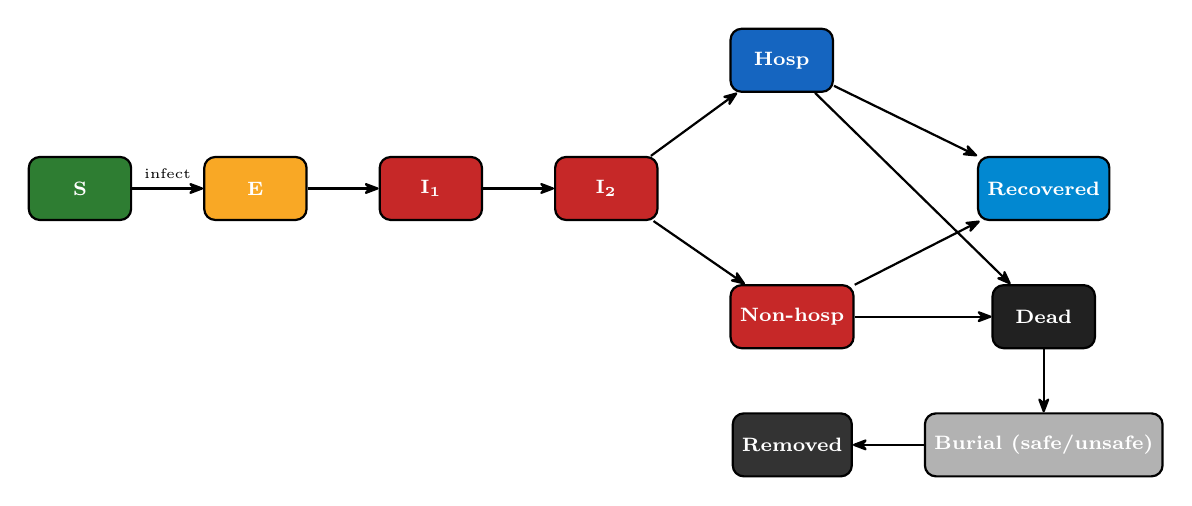
\begin{tikzpicture}[
  node distance=8mm and 9mm,
  box/.style={rectangle, rounded corners, draw, minimum height=8mm, minimum width=13mm, font=\scriptsize\bfseries, text=white},
  ->, >={Stealth[round]}, thick
]
\node[box, fill=cSus] (S) {S};
\node[box, fill=cExp, right=of S] (E) {E};
\node[box, fill=cInf, right=of E] (I1) {I\textsubscript{1}};
\node[box, fill=cInf, right=of I1] (I2) {I\textsubscript{2}};
\node[box, fill=cHosp, above right=of I2] (H) {Hosp};
\node[box, fill=cInf, below right=of I2] (N) {Non-hosp};
\node[box, fill=cRec, right=8.5cm of E] (R) {Recovered};
\node[box, fill=cDead, below=of R] (D) {Dead};
\node[box, fill=gray!60, below=of D] (B) {Burial (safe/unsafe)};
\node[box, fill=black!80, left=of B] (X) {Removed};

\draw (S) -- node[above,font=\tiny]{infect} (E);
\draw (E) -- (I1);
\draw (I1) -- (I2);
\draw (I2) -- (H);
\draw (I2) -- (N);
\draw (H) -- (R);
\draw (H) -- (D);
\draw (N) -- (R);
\draw (N) -- (D);
\draw (D) -- (B);
\draw (B) -- (X);
\end{tikzpicture}
\caption{The SEIHR/D disease state machine. Hospital-seeking, burial safety, and care delay are governed by the Information \& Trust module.}
\label{fig:seihrd}
\end{figure}

\subsection{Contagion: close contact, not casual crowds}
Ebola is not airborne; the model therefore transmits only through \emph{close contact}: household members, caregiving social ties, unsafe funerals, and health workers (under imperfect infection prevention and control). The per-contact daily hazard is
\[
p_{\text{infect}} \;=\; 1-\exp\!\big(-\beta \cdot \iota(s) \cdot d(z) \cdot \pi\big),
\]
where $\beta$ is the base transmission rate, $\iota(s)$ the infectiousness of the infector's disease state (highest for unburied bodies), $d(z)$ a crowding factor for the location, and $\pi$ a \emph{precaution} multiplier ($<1$ when the susceptible takes protective measures). $\pi$ is the key coupling: it is reduced whenever an agent correctly believes Ebola is real and is sufficiently aware---i.e.\ the information module directly throttles transmission.

\subsection{Information \& Trust module (centrepiece)}
Every agent holds beliefs (\textit{Is Ebola real? Does the hospital help? Is safe burial acceptable?}), source-specific trust (health teams, government, radio, religious/ethnic leaders), an awareness level, and a fear level. Each day:
\begin{itemize}\itemsep2pt
  \item \textbf{Radio} (e.g.\ Radio Okapi) broadcasts correct information, adopted in proportion to radio trust.
  \item \textbf{Engaged leaders} (religious/ethnic, highly trusted) push correct beliefs and safe-burial acceptance.
  \item \textbf{Rumours} spread peer-to-peer along the social network; adoption is higher when trust in health teams is low.
  \item \textbf{Survivor ambassadors} (recovered agents) and aware neighbours spread correct information and can convert rumour carriers.
  \item \textbf{Fear} rises near recent deaths and decays over time.
\end{itemize}
Belief adoption follows a trusted-information rule: an untrusted source is believed only if its message ``fits'' the agent's ethnic/religious group; a trusted source is believed unless it conflicts with a strong existing belief.

\subsection{Behaviour hooks, interventions, and context}
Beliefs and trust drive four behaviours: \emph{precautions} (transmission), \emph{hospital-seeking} (\,$p_{\text{hosp}}\propto$ trust $\times$ belief that the hospital helps\,), \emph{burial safety} (\,$p_{\text{safe}}\propto$ trust $\times$ belief $+$ safe-burial program\,), and \emph{care delay} (extended by disbelief and fear). Interventions are toggles: radio campaign, leader engagement, safe-burial program, and contact tracing (capped at the $\sim$21\% follow-up realistically achieved in the field), plus an overall RCCE-intensity dial. The population reflects Mongbwalu demographics (Lendu/Hema, miners, caregivers, health workers, $\sim$6-person households) on a spatial layout of mine, market, church, hospital, homes, and cemetery (Figure~\ref{fig:screenshot}).

\begin{figure}[h]
\centering
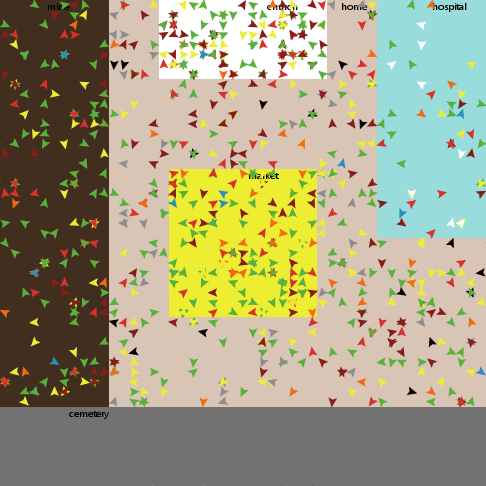
\includegraphics[width=0.62\textwidth]{figures/model_screenshot.png}
\caption{The running model (day 45). Zones: mine (brown, left), market (yellow, centre), church (white, top), hospital (blue, top-right, with hospitalised agents inside), cemetery (grey, bottom), homes (tan). Agents are coloured by disease state.}
\label{fig:screenshot}
\end{figure}

\section{Methods}
Experiments were run with NetLogo~7.0.3 BehaviorSpace via the headless launcher, 800 agents, base transmission $\beta=0.06$, each run to outbreak extinction, with \textbf{8 repetitions per condition}. End-of-run metrics: attack rate (\% ever infected), cumulative deaths, case-fatality rate (CFR), and cumulative safe vs unsafe burials.
\begin{itemize}\itemsep2pt
  \item \textbf{Experiment 1 — Misinformation gradient.} Interventions off; vary initial misinformation $\in\{0,0.25,0.5,0.75,0.9\}$ (40 runs).
  \item \textbf{Experiment 2 — Intervention impact.} Misinformation fixed at 0.6; radio, leaders, safe-burial and contact-tracing all on; vary RCCE intensity $\in\{0,0.3,0.6,0.9\}$ (32 runs).
\end{itemize}

\section{Results}

\subsection{Experiment 1: more misinformation, worse outcomes}
\begin{table}[h]
\centering
\caption{Misinformation gradient (no interventions; means of 8 runs).}
\begin{tabular}{rrrrrr}
\toprule
Init.\ misinfo & Attack \% & Deaths & CFR \% & Unsafe bur. & Safe bur. \\
\midrule
0.00 & 93.8 & 538 & 71.7 & 502 & 36 \\
0.25 & 99.4 & 599 & 75.4 & 552 & 47 \\
0.50 & 99.6 & 606 & 76.1 & 566 & 40 \\
0.75 & 99.9 & 621 & 77.8 & 576 & 45 \\
0.90 & 99.9 & 619 & 77.5 & 578 & 40 \\
\bottomrule
\end{tabular}
\label{tab:exp1}
\end{table}

\begin{figure}[h]
\centering
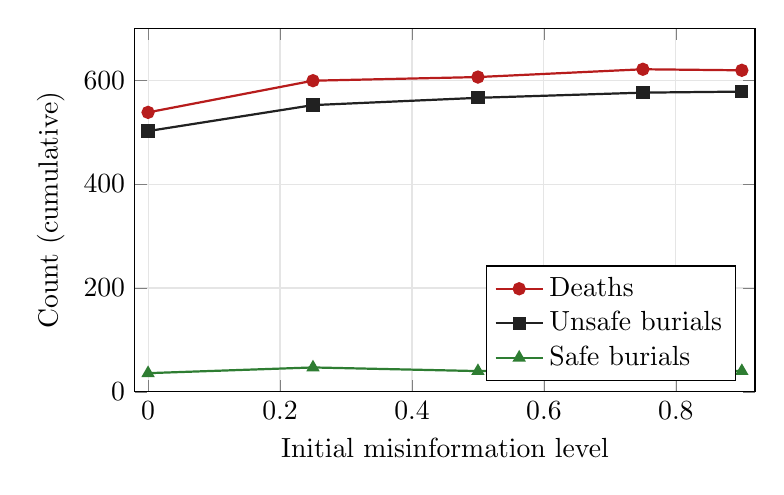
\begin{tikzpicture}
\begin{axis}[
  width=0.78\textwidth, height=6.2cm,
  xlabel={Initial misinformation level},
  ylabel={Count (cumulative)},
  xmin=-0.02, xmax=0.92,
  ymin=0, ymax=700,
  legend pos=south east, legend cell align=left,
  grid=both, grid style={gray!20},
]
\addplot[color=cAccent, mark=*, thick] coordinates {(0,538)(0.25,599)(0.5,606)(0.75,621)(0.9,619)};
\addplot[color=cDead, mark=square*, thick] coordinates {(0,502)(0.25,552)(0.5,566)(0.75,576)(0.9,578)};
\addplot[color=cSus, mark=triangle*, thick] coordinates {(0,36)(0.25,47)(0.5,40)(0.75,45)(0.9,40)};
\legend{Deaths, Unsafe burials, Safe burials}
\end{axis}
\end{tikzpicture}
\caption{Experiment 1. Rising misinformation monotonically increases deaths and unsafe burials, while safe burials stay negligible.}
\label{fig:exp1}
\end{figure}

Every increase in starting misinformation raises deaths, CFR, and unsafe burials (Table~\ref{tab:exp1}, Figure~\ref{fig:exp1}). Moving from an informed population to a heavily misinformed one adds $\sim$80 deaths and $\sim$6 CFR points; the largest single jump occurs at the first step ($0\!\to\!0.25$), showing that even a minority of misinformation materially worsens the outbreak.

\subsection{Experiment 2: trusted communication, better outcomes}
\begin{table}[h]
\centering
\caption{Intervention impact (misinformation 0.6, all interventions on; means of 8 runs).}
\begin{tabular}{rrrrrr}
\toprule
RCCE intensity & Attack \% & Deaths & CFR \% & Unsafe bur. & Safe bur. \\
\midrule
0.0 & 99.5 & 611 & 76.8 & 570 & 42 \\
0.3 & 97.2 & 554 & 71.2 & 388 & 166 \\
0.6 & 95.3 & 521 & 68.3 & 270 & 250 \\
0.9 & 89.7 & 467 & 65.0 & 159 & 307 \\
\bottomrule
\end{tabular}
\label{tab:exp2}
\end{table}

\begin{figure}[h]
\centering
\begin{subfigure}{0.49\textwidth}
\centering
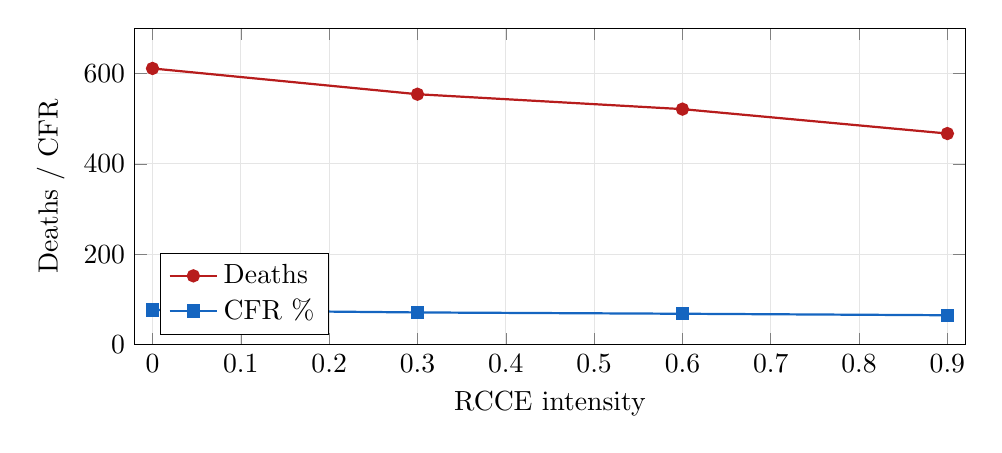
\begin{tikzpicture}
\begin{axis}[
  width=\textwidth, height=5.6cm,
  xlabel={RCCE intensity}, ylabel={Deaths / CFR},
  xmin=-0.02, xmax=0.92, ymin=0, ymax=700,
  legend pos=south west, legend cell align=left,
  grid=both, grid style={gray!20},
]
\addplot[color=cAccent, mark=*, thick] coordinates {(0,611)(0.3,554)(0.6,521)(0.9,467)};
\addplot[color=cHosp, mark=square*, thick] coordinates {(0,76.8)(0.3,71.2)(0.6,68.3)(0.9,65.0)};
\legend{Deaths, CFR \%}
\end{axis}
\end{tikzpicture}
\caption{Deaths and case-fatality fall.}
\end{subfigure}\hfill
\begin{subfigure}{0.49\textwidth}
\centering
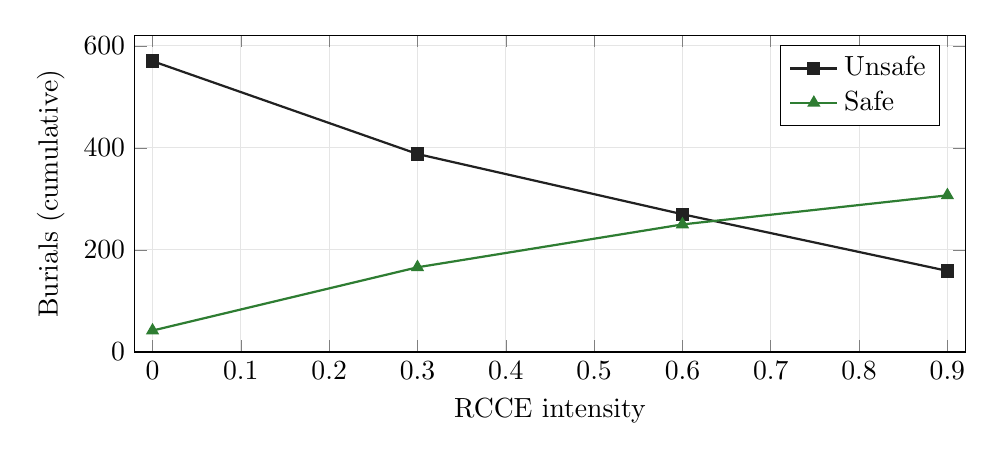
\begin{tikzpicture}
\begin{axis}[
  width=\textwidth, height=5.6cm,
  xlabel={RCCE intensity}, ylabel={Burials (cumulative)},
  xmin=-0.02, xmax=0.92, ymin=0, ymax=620,
  legend pos=north east, legend cell align=left,
  grid=both, grid style={gray!20},
]
\addplot[color=cDead, mark=square*, thick] coordinates {(0,570)(0.3,388)(0.6,270)(0.9,159)};
\addplot[color=cSus, mark=triangle*, thick] coordinates {(0,42)(0.3,166)(0.6,250)(0.9,307)};
\legend{Unsafe, Safe}
\end{axis}
\end{tikzpicture}
\caption{Burials flip safe.}
\end{subfigure}
\caption{Experiment 2. As trusted-communication intensity rises, deaths and CFR fall monotonically (a) and burials cross over from majority unsafe to majority safe between intensity 0.3 and 0.6 (b).}
\label{fig:exp2}
\end{figure}

Raising RCCE intensity produces a clean dose--response (Table~\ref{tab:exp2}, Figure~\ref{fig:exp2}): deaths fall $\sim$24\% (611$\to$467), CFR falls $\sim$12 points (76.8\%$\to$65.0\%), the attack rate falls $\sim$10 points, and burials flip from 570 unsafe / 42 safe to 159 unsafe / 307 safe. The burial crossover---the single most movable lever---occurs between intensity 0.3 and 0.6.

\section{Discussion}
\textbf{Information is an intervention.} With no vaccine or drug for Bundibugyo, the model shows that what people believe and whom they trust is a primary determinant of mortality. \textbf{Trusted channels matter.} Effects flow through trust: radio, religious/ethnic leaders, and survivor ambassadors. \textbf{Safe burial is the most responsive lever}, consistent with funerals being a dominant EVD transmission route. \textbf{Harm reduction is achievable even when elimination is not}: strong intervention does not drive the attack rate to zero (it falls from $\sim$99\% to $\sim$90\%); eliminating transmission additionally requires earlier and stronger case isolation to push the reproduction number below one.

\section{Limitations}
The model is a single, well-connected community, so attack rates run high (standard susceptible--infectious--recovered behaviour once the pathogen is seeded); geographic and social fragmentation would lower totals. CFR is higher than the $\sim$17\% Bundibugyo headline because the no-intervention baseline involves almost no hospitalisation; it falls as care-seeking rises and is tunable. Parameters are plausible and data-informed but not yet formally calibrated to the 15--23 May 2026 line list, and belief updating is rule-based rather than learned.

\section{Conclusion and future work}
A behaviour-rich ABM of the 2026 Bundibugyo outbreak shows, with clean monotonic evidence, that misinformation worsens and trusted communication improves outbreak outcomes---especially deaths and burial safety. Next steps: (i) calibrate to the May~2026 line list; (ii) model Hema/Lendu trust asymmetry and differential clinic access; (iii) replace rule-based belief updating with LLM-driven, persona-level reasoning and feed a real-data misinformation-monitoring pipeline into the model's rumour sources; and (iv) port the Information \& Trust module into the ASSOCC Ebola codebase.

\paragraph{Reproducibility.} Model: \texttt{Ebola\_Mongbwalu\_InformationTrust.nlogox}. Experiment~1: 40 runs (8 reps $\times$ 5 misinformation levels, interventions off). Experiment~2: 32 runs (8 reps $\times$ 4 RCCE levels, all interventions on, misinformation 0.6). Raw tables: \texttt{exp1\_misinformation\_gradient\_*.table.csv}, \texttt{exp2\_intervention\_impact\_*.table.csv}. Engine: NetLogo 7.0.3 BehaviorSpace (headless), driven via the NetLogo MCP server.

\begin{thebibliography}{9}
\bibitem{who2026} World Health Organization. \emph{Ebola disease caused by Bundibugyo virus -- Democratic Republic of the Congo and Uganda.} Disease Outbreak News, 2026.
\bibitem{cdc2026} U.S.\ Centers for Disease Control and Prevention. \emph{Ebola Disease Outbreak in the DRC and Uganda.} Health Alert Network (HAN-00530), 2026.
\bibitem{assocc} Dignum, F.\ et al. \emph{Agent-Based Social Simulation of the Coronavirus Crisis (ASSOCC).} \url{https://github.com/lvanhee/COVID-sim}, 2020.
\bibitem{weitz2015} Weitz, J.S., Dushoff, J. \emph{Modeling post-death transmission of Ebola: challenges for inference and opportunities for control.} Scientific Reports, 2015.
\bibitem{merler2015} Merler, S.\ et al. \emph{Spatiotemporal spread of the 2014 outbreak of Ebola virus disease in Liberia and the effectiveness of interventions: an agent-based model.} The Lancet Infectious Diseases, 2015.
\bibitem{funk2015} Funk, S.\ et al. \emph{The role of human behaviour in the transmission dynamics of Ebola virus disease.} (behaviour-change incidence models), 2015.
\end{thebibliography}

\end{document}
